% ------------------------------------------------------------------
\renewcommand{\thisunit}{MATH327 Unit 9}
\renewcommand{\moddate}{Last modified 12 May 2023}
\setcounter{section}{9}
\setcounter{subsection}{0}
\phantomsection
\addcontentsline{toc}{section}{Unit 9: Interacting systems}
\section*{Unit 9: Interacting systems}
\subsection{\label{sec:Ising}The Ising model}
So far in this module we have considered `ideal' systems composed of constituent degrees of freedom that do not interact with each other.
While we have seen that this approximation of non-interacting particles can produce excellent mathematical models for real physical systems ranging from the low-temperature heat capacities of solids to solar radiation and the cosmic microwave background, there are crucial statistical physics phenomena that this approach fails to predict.

An important class of examples, which we investigate in this unit, are \textit{phase transitions}.
These occur when interactions allow extremely different large-scale behaviours to arise from the same set of degrees of freedom, depending on control parameters such as the temperature or pressure.
Phase transitions occur in both everyday and extreme situations.
Everyday examples include the liquid--gas transition of H$_2$O molecules from water to steam upon boiling a kettle, as well as the transition from liquid water to solid ice as the temperature decreases.
In the extreme conditions following the big bang, the matter in the universe existed as a charged plasma of quarks and gluons.
Once the universe was a few micro-seconds old, it cooled enough for this matter to transition into the protons and neutrons we are made out of today. % TODO: Crossover vs. phase transition depends on quark masses...

An intermediate example in between the everyday and the extreme involves two layers of graphene as illustrated in the figure below.\footnote{Heather M. Hill, ``\href{https://doi.org/10.1063/PT.3.4384}{Twisted bilayer graphene enters a new phase}'', \textit{Physics Today} \textbf{73}:18, 2020.}
Graphene is an amazing material (recognized by the 2010 Nobel Prize in Physics) that consists of a single-atom-thick sheet of carbon atoms arranged in a hexagonal `honeycomb' lattice.
Under most conditions, graphene is an electrical insulator.
However, if two graphene sheets are stacked and rotated with respect to each other by a small ``magic angle'' $\theta \approx 1.1^{\circ}$, the system transitions into a superconducting phase at low temperatures $T \lesssim 1.7$~K.
Superconductivity allows electrical current to flow with no resistance, meaning that no energy is lost to the production of waste heat.
If we could discover or design materials that exhibit superconductivity at everyday temperatures $T \sim 300$~K rather than low $T \sim \cO(1)$~K, it would revolutionize the energy efficiency of electronics and the power grid.

\begin{center}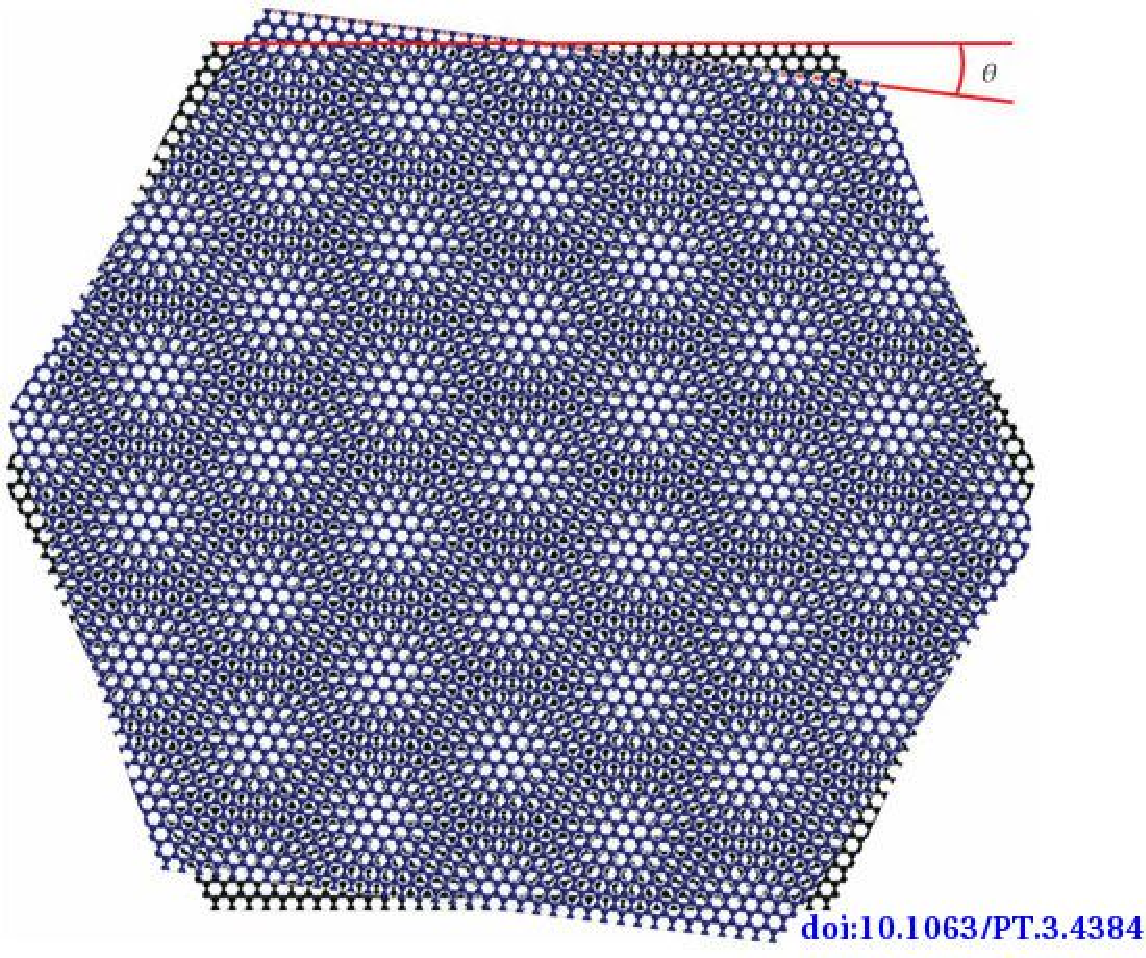
\includegraphics[width=0.45\textwidth]{figs/unit09_graphene.pdf}\end{center} % WARNING: ADJUSTED SIZE BY HAND TO FILL REMAINDER OF PAGE

With this motivation for investigating phase transitions, let's step back to introduce interactions and explore their effects using simple spin systems of the sort we considered in units $2$ and $3$.
In the non-interacting case we previously analyzed (\eq{eq:spin_energy}), the internal energy of the system is
\begin{equation*}
  E_i = -H \sum_{n = 1}^N s_n \qquad \mbox{(non-interacting)}
\end{equation*}
for micro-state $\om_i$ specified by the $N$ spins $\left\{s_n\right\}$ (and, as always for this module, in thermodynamic equilibrium).
Here $H > 0$ is the constant strength of an external magnetic field and the orientation of the $n$th spin, $s_n$, takes one of only two possible values: $s_n = 1$ if the spin is aligned parallel to the field and $s_n = -1$ if the spin is aligned anti-parallel to the field.
The ground state of the system features all $N$ spins aligned parallel to the magnetic field, with minimal energy $E_0 = -NH$.

In this unit we will only consider systems of distinguishable spins that we label by their fixed position in a $d$-dimensional simple cubic \textbf{lattice}.
The $d = 1$ case of a one-dimensional lattice is precisely the system of spins arranged in a line that we analyzed in \secref{sec:spin_chain}.
This and the case of $d = 2$ are both easy to visualize and draw on a sheet of paper:
\begin{mdframed}
  \ \\[100 pt]
\end{mdframed}
While we can only have physical lattices with $d = 1$, $2$ or $3$ in nature, the mathematical construction works just as well for any integer $d \geq 1$.

We can see that the total internal energy of the non-interacting system can easily be written as a sum over energies $\eps_n$ for each individual spin,
\begin{align*}
  \eps_n & = -H s_n &
  E_i & = \sum_{n = 1}^N \eps_n \qquad \mbox{(non-interacting)}.
\end{align*}
This is a generic feature of non-interacting systems, and an aspect of the \textbf{factorization} that enormously simplifies calculations --- in this case by causing the $N$-particle partition function (\eq{eq:spin_part_func}) to take the form of a product of $N$ identical terms, $Z_N = \left[2\cosh\left(\be H\right)\right]^N = Z_1^N$.
However, it is possible to have non-factorizable systems in which the internal energy can be expressed as a sum of this sort.
A stronger condition needs to be satisfied in order to guarantee factorization, and this conditions rigorously defines what it means for a system to be non-interacting.

\begin{shaded}
  Let $\De E_j$ be the change in the system's internal energy caused by changing its $j$th degree of freedom.
  Then the system is defined to be \textbf{non-interacting} if and only if $\De E_j$ is independent of all other degrees of freedom $k \ne j$. % for an arbitrary $j$...
\end{shaded}

For our system of $N$ distinguishable spins, the only possible change we can make to a degree of freedom is to negate it, $s_j \to -s_j$, which corresponds to flipping its alignment relative to the external magnetic field.
It is easy to check that the change in the internal energy resulting from such a spin flip satisfies our definition of a non-interacting system:
\begin{mdframed}
  \ \\[80 pt]
\end{mdframed}

Now let's make things more interesting by considering a different spin system that includes a simple two-spin contribution to the internal energy:
\begin{equation}
  \label{eq:Ising_energy}
  E_i = -\sum_{(jk)} s_j s_k - H \sum_{n = 1}^N s_n.
\end{equation}
The first sum runs over all pairs of nearest-neighbour spins in the lattice, denoted $(jk)$.
What is the change in energy $\De E_j$ from \eq{eq:Ising_energy} upon negating $s_j \to -s_j$?
Does this indicate an interacting or non-interacting system?
\begin{mdframed}
  \ \\[100 pt]
\end{mdframed}

The pictures on the next page illustrate nearest-neighbour pairs for simple cubic lattices in $d = 2$ and $3$ dimensions, while also introducing some additional lattice terminology.
Instead of drawing up- and down-pointing arrows, these pictures identify the spins with \textit{sites} in the lattice represented as points (or larger filled circles).
In simple cubic lattices, all sites are positioned in a regular grid, separated by a constant distance along each basis vector.
We can also draw \textit{links} as solid lines connecting these nearest-neighbour sites, with each link corresponding to a term in $\sum_{(jk)}$.
The picture of a two-dimensional lattice on the left highlights the four links (with red hatch marks) that correspond to the four nearest neighbours (circled in red) of a particular site (circled in blue).
For $d \geq 2$, the elementary unit of surface area is called a \textit{plaquette}, while for $d \geq 3$ the elementary unit of volume is called a \textit{cube}.

\begin{center}
  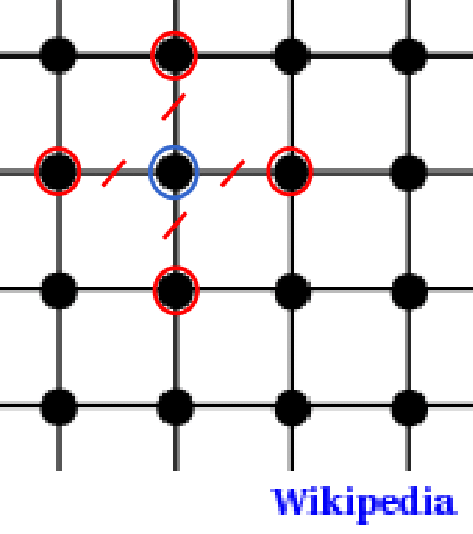
\includegraphics[height=0.4\textwidth]{figs/unit09_lattice_2d.pdf}\hfill
  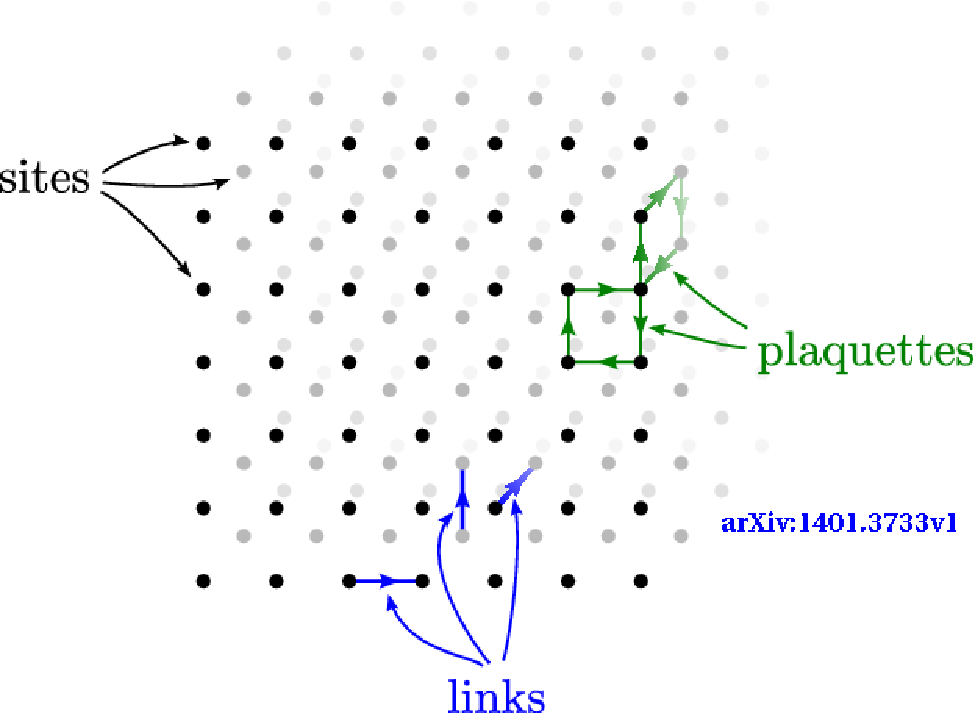
\includegraphics[height=0.4\textwidth]{figs/unit09_lattice_3d.pdf}
\end{center}

Computing the energy in \eq{eq:Ising_energy} requires determining all of the nearest-neighbour pairs to be summed in the first term, which is equivalent to all of the links in the lattice, $\ell = (jk)$.
When considering a finite lattice, this task is complicated by the need to consider the edges of the lattice.
We can avoid this complication by imposing \textbf{periodic boundary conditions}, which remove these edges by adding links between each site on the left edge of the lattice and the corresponding site on the right edge, and similarly in all other dimensions.
This is illustrated below for the simple case of the one-dimensional lattice, drawn as a circle to emphasize that all $N$ sites remain separated by a constant distance.
In higher dimensions, periodic boundary conditions produce flat (zero-curvature) $d$-dimensional tori that preserve the simple cubic lattice structure. \\[-24 pt]
\begin{center}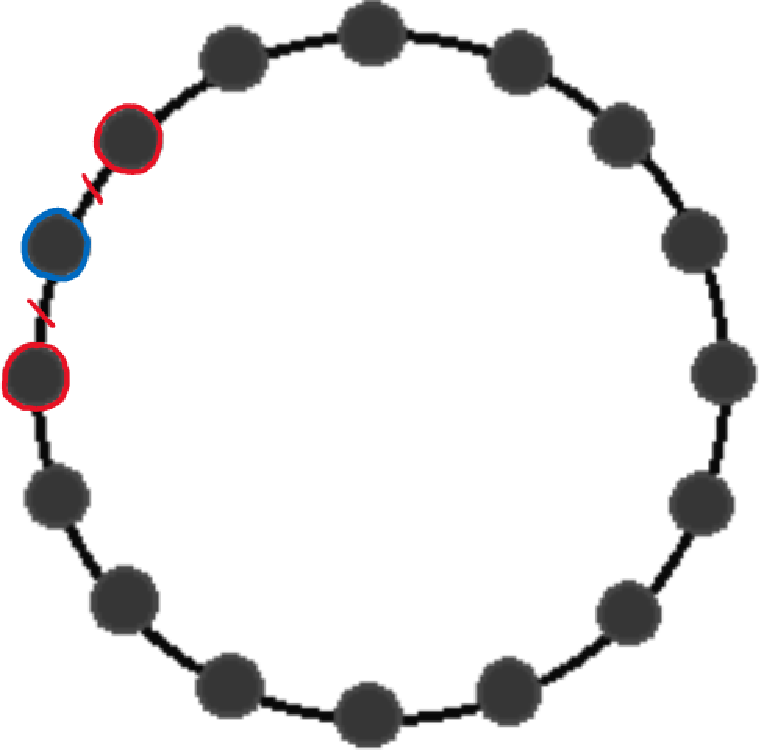
\includegraphics[width=0.425\textwidth]{figs/unit09_lattice_1d.pdf}\end{center} % WARNING: ADJUSTED SPACING AND SIZE BY HAND TO KEEP NEXT TWO SENTENCES ON THIS PAGE

With periodic boundary conditions, we can easily see that the $N$-site one-dimensional lattice drawn above has $N$ links.
Each site has two links connecting it to its two nearest neighbours, and each of those links is shared between two sites, so that $\#\ell = 2N / 2 = N$.
Looking back to the two-dimensional lattice drawn farther above, the four links per site produce $\#\ell = 4N / 2 = 2N$.
How many terms are there in the sum $\sum_{(jk)}$ in \eq{eq:Ising_energy} for $N$-site lattices with periodic boundary conditions in $d$ dimensions?
\begin{mdframed}
  \ \\[50 pt]
\end{mdframed}

The energy of interacting spins given by \eq{eq:Ising_energy}, with a lattice structure defined to specify which spins form the nearest-neighbour pairs $(jk)$, defines a famous system known as the $d$-dimensional \textbf{Ising model}.
Since the 1960s, the Ising model has been the basis of thousands of scientific studies analyzing everything from ferromagnetism to neural networks to urban segregation.\footnote{For a brief discussion, see Charlie Wood, ``\href{https://www.quantamagazine.org/the-cartoon-picture-of-magnets-that-has-transformed-science-20200624/}{The Cartoon Picture of Magnets That Has Transformed Science}'', \textit{Quanta Magazine}, 2020.}
The model was proposed in 1920 by \href{https://en.wikipedia.org/wiki/Wilhelm_Lenz}{Wilhelm Lenz}, whose PhD student \href{https://en.wikipedia.org/wiki/Ernst_Ising}{Ernst Ising} solved the one-dimensional system as a research project in 1924.
Exactly solving the two-dimensional case (with $H = 0$) took another twenty years, culminating in renowned work by \href{https://en.wikipedia.org/wiki/Lars_Onsager}{Lars Onsager} in 1944.
The three-dimensional Ising model remains an open mathematical question, with no known exact solution.

In this context, `solving' the Ising model means deriving a closed-form expression for its canonical partition function,
\begin{equation*}
  Z(\be, N, H) = \sum_{\left\{s_n\right\}} \exp\left[-\be E(s_n)\right] = \sum_{\left\{s_n\right\}} \exp\left[\be\sum_{(jk)} s_j s_k + \be H \sum_n s_n\right].
\end{equation*}
As in \secref{sec:spin_info}, the partition function sums over all possible spin configurations $\left\{s_n\right\}$, which amounts to a sum of $2^N$ exponential factors for $N$ spins, with $\cO(N)$ terms within each exponential.
Now that the system is interacting, the partition function no longer factorizes into the $N$ identical $\cosh$ factors of \eq{eq:spin_part_func}, making it extremely difficult to evaluate.
This is why there is no known exact solution to the three-dimensional Ising model, and it also makes `brute-force' numerical computations impractical.
Even for a system of $N = 1023$ spins, twenty orders of magnitude smaller than our typical $N \sim 10^{23}$, there are roughly $2^{1023} \sim 10^{310}$ terms in the partition function, far beyond the capabilities of existing or foreseeable supercomputers.
% ------------------------------------------------------------------



% ------------------------------------------------------------------
\subsection{\label{sec:Ising_phases}Ising model phases and phase transition}
Despite the insolubility of the Ising model in an arbitrary number of $d$ dimensions, we can still make robust predictions for its large-scale behaviour by considering the simplified limits of high and low temperature, much as we did for non-interacting spin systems in \secref{sec:spin_info}.
We can also simplify the system by setting $H = 0$ in this section, and considering just
\begin{align}
  \label{eq:Ising_zero_field}
  E_i & = -\sum_{(jk)} s_j s_k &
  Z(\be, N) & = \sum_{\left\{s_n\right\}} \exp\left[\be\sum_{(jk)} s_j s_k\right].
\end{align}
We will see that the behaviour of this zero-field Ising model is qualitatively different at high temperatures compared to low temperatures.
In other words, the system exhibits at least two distinct phases for different temperatures.
This is a necessary but not sufficient condition for there to be a true phase transition --- it leaves open the possibility of a gradual \textit{crossover} between these two phases, as opposed to a rapid transition.
In this section we will use the Ising model to more rigorously define what exactly constitutes a phase transition, and how this can be distinguished from a crossover.

First, though, let's consider the \textbf{high-temperature} limit $\be \to 0$, where the Ising model partition function becomes extremely simple:
\begin{mdframed}
  $\displaystyle \lim_{\be \to 0} Z(\be, N) = $ \\[40 pt]
\end{mdframed}
In this limit, all $2^N$ spin configurations are adopted with the same probability $p_i = 1 / 2^N$, regardless of their internal energy from \eq{eq:Ising_zero_field}.
In effect, that energy has become negligible compared to the temperature.

Rather than computing the expectation value of that internal energy, there is a simpler observable that we can consider to characterize this high-temperature phase.
This is the \textbf{magnetization} $M = n_+ - n_-$, retaining our definition of $n_{\pm}$ as the number of spins with value $\pm 1$, even without an external field for them to align with or align against.
It is convenient to normalize the magnetization by the number of spins,
\begin{equation}
  \label{eq:Ising_magnet}
  m \equiv \frac{M}{N} = \frac{n_+ - n_-}{n_+ + n_-},
\end{equation}
so that $-1 \leq m \leq 1$ for any value of $N$.
In addition, without an external field to distinguish between $\pm 1$ spins, it is also convenient to consider the absolute magnitude $0 \leq |m| \leq 1$.

Our task is now to determine the expectation value of the magnetization at high temperatures.
Above we found that all spin configurations are equally probable in this regime, so $\vev{|m|}$ will be determined by how many of these equally-probably micro-states have a particular magnetization.
For example, there are only two micro-states with $|m| = 1$, corresponding to $(n_+, n_-) = (N, 0)$ and $(0, N)$.
In general, just as we saw in \eq{eq:spin_states}, there are
\begin{equation*}
  \binom{N}{n_+} = \binom{N}{n_-} = \frac{N!}{n_+! \; n_-!}
\end{equation*}
equally probable micro-states with a given $n_+ = N - n_-$.
For large $N \gg 1$ this binomial coefficient has a factorially narrow peak around
\begin{equation*}
  n_+ = n_- = \frac{1}{2} N \qquad \lra \qquad |m| = 0.
\end{equation*}
This characterizes a \textbf{disordered phase} with similar numbers of up- and down-pointing spins producing a small magnetization.
In the \textit{thermodynamic limit} $N \to \infty$, the expectation value of the magnetization in the disordered phase vanishes exactly, $\vev{|m|} \to 0$.

We next need to determine $\vev{|m|}$ in the \textbf{low-temperature} limit $\be \to \infty$.
In this regime, as we saw in \secref{sec:spin_chain}, the Boltzmann factor $\exp\left[\be\sum_{(jk)} s_j s_k\right]$ makes it exponentially more likely for the system to adopt micro-states with lower energies.
In particular, we can expect the ground state to dominate the expectation value of the magnetization, $\vev{|m|}$, up to exponentially suppressed corrections from higher-energy excited states.
With $H = 0$, the Ising model has two degenerate ground states corresponding to the two ways all the spins can be aligned with each other: $(n_+, n_-) = (N, 0)$ and $(0, N)$.
What is the ground-state energy of the $N$-site Ising model in $d$ dimensions?
\begin{mdframed}
  $\displaystyle E_0 = -\sum_{(jk)} s_j s_k = $ \\[50 pt]
\end{mdframed}

As mentioned above, both of these degenerate ground states have the maximal magnetization $|m| = 1$.
Let's check what effect the first excited state would have on the overall magnetization of the system.
For $d > 1$, the first excited energy level is obtained by flipping a single spin --- negating its value.
Starting from the two degenerate ground states, this produces all possible micro-states with $(n_+, n_-) = (N - 1, 1)$ and $(1, N - 1)$.
Because any one of the $N$ spins in the lattice could be flipped, the degeneracy of this first excited energy level grows with $N$:
\begin{equation*}
  \binom{N}{1} + \binom{N}{N - 1} = 2N.
\end{equation*}
At the same time, as $N$ increases the magnetization of each of these micro-states gets closer to that of the ground state,
\begin{equation*}
  |m| = \frac{N - 2}{N} = 1 - \frac{2}{N}.
\end{equation*}
\newpage % WARNING: FORMATTING BY HAND
\noindent The key factor is the probability for the system to be in one of these micro-states, which depends on the value of the energy $E_1$ for the first excited energy level.
What is this $E_1$ for the $N$-site Ising model in $d$ dimensions?
\begin{mdframed}
  $\displaystyle E_1 = $ \\[100 pt]
\end{mdframed}

Let's bring everything together by computing the relative probability for the $d$-dimensional Ising model to be in its ground state with $|m| = 1$ compared to its first excited state with $|m| = 1 - \frac{2}{N}$.
We just need to multiply the degeneracy of each energy level times the corresponding Boltzmann factor for each degenerate micro-state, while the $\frac{1}{Z}$ normalization cancels out in the ratio
\begin{equation*}
  \frac{P(E_0)}{P(E_1)} = \frac{2\cdot \exp\left[\be d\cdot N\right]}{2N\cdot \exp\left[\be \left(d\cdot N - 4d\right)\right]} = \frac{\exp\left[4\be d\right]}{N}.
\end{equation*}
For any fixed $N$, a sufficiently low temperature will cause the ground state to dominate, with exponentially suppressed contributions from higher energy levels, just as we previously found for simpler non-interacting systems.
This characterizes an \textbf{ordered phase} with essentially all spins aligned in the same direction, producing a large expectation value for the magnetization, $\vev{|m|} \to 1$.

We have now seen how the behaviour of the magnetization $\vev{|m|}$ distinguishes the high- and low-temperature phases of the zero-field Ising model in $d > 1$ dimensions.
In the high-temperature disordered phase, the magnetization is small and $\vev{|m|} \to 0$ in the thermodynamic limit $N \to \infty$.
In the low-temperature ordered phase, the magnetization is large and $\vev{|m|} \to 1$ as $T \to 0$.

This contrast between ordered and disordered phases is typical behaviour for interacting statistical systems.
These two phases are distinguished by an \textbf{order parameter} --- an observable (related to a derivative of the free energy) that is zero in the disordered phase but non-zero in the ordered phase.\footnote{There are atypical (but interesting and important) \textit{topological phase transitions} that are not characterized by such an order parameter.  The most famous example is the BKT phase transition named after \href{https://en.wikipedia.org/wiki/Vadim_Berezinskii}{Vadim Berezinskii}, \href{https://en.wikipedia.org/wiki/J._Michael_Kosterlitz}{J.\ Michael Kosterlitz} and \href{https://en.wikipedia.org/wiki/David_J._Thouless}{David Thouless}, which was awarded the 2016 Nobel Prize in Physics.  It is also possible for a single system to have multiple distinct phase transitions, each characterized by a different order parameter.}
The magnetization is the order parameter for the Ising model, which we will connect to the free energy in the next section.
Note that the order parameter need not reach its maximum value in the ordered phase --- in the case of the Ising model, we don't need complete domination by the fully ordered ground state.
So long as there is a tendency towards order, mathematically defined by a non-zero order parameter, the system is in the ordered phase.
The details of how the order parameter changes between zero and non-zero values are what distinguish gradual crossovers from rapid phase transitions.

\begin{shaded}
  A \textbf{phase transition} is defined by a discontinuity or divergence in the order parameter or its derivative(s), in the $N \to \infty$ thermodynamic limit.
  The value(s) of the control parameter(s) at which the discontinuity occurs define the \textit{critical point} corresponding to the transition.
\end{shaded}

For the zero-field Ising model, since we have set $H = 0$, the only remaining control parameter is the temperature $T$.
Any phase transition would therefore occur at a \textbf{critical temperature} $T_C$.
The sketches below illustrate the most common types of phase transitions.
When the order parameter (OP) itself is discontinuous (shown by a dashed line), the transition is said to be a \textit{first-order} phase transition. % TODO: Leads to non-zero latent heat...
When the order parameter is continuous at $T_C$ but its first derivative with respect to the control parameter is discontinuous (typically divergent), the transition is said to be a \textit{second-order} phase transition.
Historically, this naming scheme was extended to $n$th-order phase transitions for which discontinuities don't occur until the $(n-1)$th derivative of the order parameter (related to an $n$th derivative of the free energy).
At present it is more common for any phase transition with a continuous order parameter to be called simply a second-order transition.

\begin{center}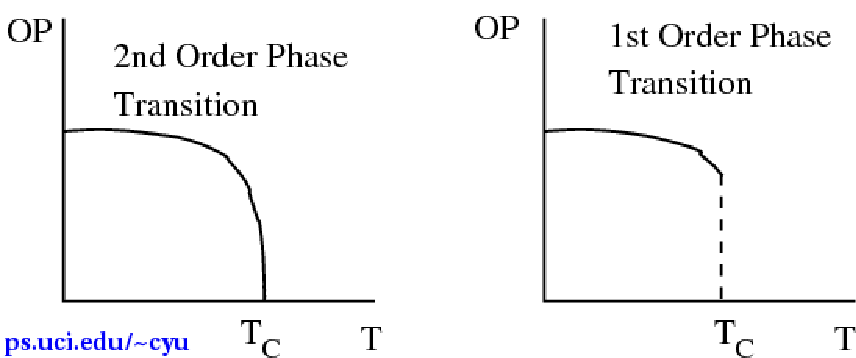
\includegraphics[width=0.8\textwidth]{figs/unit09_transitions.pdf}\end{center}

In practice, any system with a finite number of degrees of freedom will not exhibit a true discontinuity or divergence in any observable.
As a result, it is sometimes said that true phase transitions only occur in the $N \to \infty$ thermodynamic limit, but I consider this excessively pedantic, especially given the finite number of atoms in the observable universe.
We are still able to distinguish crossovers from true phase transitions when considering a finite number of degrees of freedom, by analyzing the way in which the system approaches the thermodynomic limit.
If there is time and inclination, we may explore such \textit{finite-size scaling}, but first we will develop a useful approximation technique, and apply it to the Ising model to investigate its (dimensionality-dependent) phase transition in more detail.
% ------------------------------------------------------------------



% ------------------------------------------------------------------
\subsection{\label{sec:mean_field}The mean-field approximation}
Having identified the ordered and disordered phases of the zero-field Ising model, respectively at low and high temperatures, let's now restore a non-zero external magnetic field, $H > 0$.
This will allow us to gain a deeper appreciation of the magnetization --- now with no absolute value --- by noting that \eq{eq:Ising_magnet} means the magnetization is just the average spin:
\begin{equation*}
  m = \frac{M}{N} = \frac{1}{N}\left(n_+ - n_-\right) = \frac{1}{N} \sum_{n = 1}^N s_n.
\end{equation*}
We can benefit from this observation in two ways.
First, we can recognize the magnetization in the internal energy of the full Ising model with $H >0$:
\begin{equation*}
  E_i = -\sum_{(jk)} s_j s_k - H \sum_{n = 1}^N s_n = -\sum_{(jk)} s_j s_k - H N m = -\sum_{(jk)} s_j s_k - H M.
\end{equation*}
The corresponding canonical partition function is
\begin{equation*}
  Z = \sum_{\left\{s_n\right\}} \exp\left[\be \sum_{(jk)} s_j s_k + \be H M\right].
\end{equation*}
Based on this expression, and our earlier experience with the entropy and internal energy, we can anticipate that $\vev{m} = \vev{M} / N$ is related to the derivative of the Helmholtz free energy $F = -T\log Z$ with respect to the field strength $H$:
\begin{mdframed}
  $\displaystyle \pderiv{}{H} F = $ \\[100 pt]
\end{mdframed}
As promised in the previous section, this relation ensures that the magnetization is an appropriate order parameter for the Ising model phase transition.

The second way we can benefit from relating the magnetization to the average spin is to express the Ising model in terms of the expectation value
\begin{equation*}
  \vev{m} = \frac{1}{Z} \sum_{\left\{s_n\right\}} m \; e^{-\be E(s_n)} = \frac{1}{N} \sum_{n = 1}^N \vev{s_n}.
\end{equation*}
The expectation value of the average spin, $\frac{1}{N} \sum_{n = 1}^N \vev{s_n}$, is independent of the spin configuration $\left\{s_n\right\}$ and is simply a function of the inverse temperature \be and magnetic field strength $H$.
By adding and subtracting factors of $\vev{m}$, we can exactly rewrite each nearest-neighbour term in the Ising model energy, \eq{eq:Ising_energy}, as
\begin{align}
  s_j s_k & = \left[\left(s_j - \vev{m}\right) + \vev{m}\right] \times \left[\left(s_k - \vev{m}\right) + \vev{m}\right] \cr
          & = \left(s_j - \vev{m}\right) \left(s_k - \vev{m}\right) + \left(s_j + s_k\right)\vev{m} + \vev{m}^2. \label{eq:MF_start}
\end{align}

This is beneficial because we can note that the factors of $\left(s_j - \vev{m}\right)$ correspond to the spins' fluctuations around their mean value $\vev{m}$.
By conjecturing that these fluctuations are small \textit{on average}, we can approximate the Ising model energy by neglecting the first term in \eq{eq:MF_start} when summing over all links:
\begin{equation*}
  E_i = -\sum_{(jk)} s_j s_k - H \sum_{n = 1}^N s_n \quad \lra \quad \EMF = -\sum_{(jk)} \left[\left(s_j + s_k\right)\vev{m} + \vev{m}^2\right] - H \sum_{n = 1}^N s_n.
\end{equation*}
The sum over the links $\ell = (jk)$ in $d$ dimensions simply counts $d\cdot N$ factors of the constant $\vev{m}^2$.
Similarly, since the first term includes both spins $\left(s_j + s_k\right)$ on each end of the link, every individual spin appears $2d$ times in the sum over links.
Therefore this term just gives us $2d\vev{m}$ times another sum over the spins $s_n$, which we can combine with the final term above:
\begin{equation}
  \label{eq:MF_energy}
  \EMF = -d\cdot N \vev{m}^2 - \left(2d\vev{m} + H\right) \sum_{n = 1}^N s_n \equiv -d\cdot N \vev{m}^2 - H_{\text{eff}} \sum_{n = 1}^N s_n.
\end{equation}

In this expression we define an effective magnetic field $H_{\text{eff}} = 2d\vev{m} + H$ that depends on the mean spin.
This is a way to remember that this approach of neglecting the squared fluctuations $\left(s_j - \vev{m}\right) \left(s_k - \vev{m}\right)$ is known as the \textbf{mean-field approximation}.
In essence, this approach supposes that we can average over all $2d$ nearest neighbours of each spin and end up with an approximately constant factor that behaves like a modification of the magnetic field. % TODO: Applies more generally than just the Ising model...
Given the resulting mean-field energy \EMF from \eq{eq:MF_energy}, let's check the change in this energy, $\De E_j$, upon negating any $s_j \to -s_j$:
\begin{mdframed}
  \ \\[120 pt]
\end{mdframed}

\newpage % WARNING: FORMATTING BY HAND
In light of this result, it isn't surprising that the mean-field approximation producing \eq{eq:MF_energy} makes it very easy to compute the corresponding canonical partition function
\begin{align}
  \ZMF & = \sum_{\left\{s_n\right\}} \exp\left[-\be E(s_n)\right] = \exp\left[\be d\cdot N \vev{m}^2\right] \sum_{s_1 = \pm 1} \cdots \sum_{s_N = \pm 1} \exp\left[-x \sum_{n = 1}^N s_n\right] \cr
       & = \exp\left[\be d\cdot N \vev{m}^2\right] \left(2\cosh\left[\be H_{\text{eff}}\right]\right)^N \nonumber \\
       & = \exp\left[\be d\cdot N \vev{m}^2\right] \left(2\cosh\left[\be \left(2d\vev{m} + H\right)\right]\right)^N,
\end{align}
where we defined $x \equiv -\be H_{\text{eff}}$ to put the sums into the same form as in \eq{eq:spin_part_func}.
Although this factorized result is far simpler than the partition function for the full Ising model, it does involve some complicated dependence on $\vev{m}$ --- especially when we recall that $\vev{m}$ itself is related to a derivative of $\log \ZMF$. % TODO: $\vev{m}$ is now essentially both degree of freedom and prediction...
With
\begin{equation*}
  \log \ZMF = N\log \cosh\left[\be \left(2d\vev{m} + H\right)\right] + \left\{H\mbox{-independent terms}\right\},
\end{equation*}
the relation we derived above gives us
\begin{equation*}
  \vev{m} = \frac{1}{N\be} \pderiv{}{H}\log \ZMF = \frac{1}{\be} \frac{1}{\cosh\left[\be \left(2d\vev{m} + H\right)\right]} \pderiv{}{H}\cosh\left[\be \left(2d\vev{m} + H\right)\right].
\end{equation*}
Simplifying, we obtain a \textbf{self-consistency condition} for the Ising model magnetization in the mean-field approximation:
\begin{equation}
  \label{eq:consistency}
  \vev{m} = \tanh\left[\be \left(2d\vev{m} + H\right)\right].
\end{equation}
Solving this equation for $\vev{m}$ is equivalent to finding the roots of the equation $\tanh\left[\be (2d\cdot x + H)\right] - x = 0$.

A straightforward way to inspect such solutions is by plotting both
\begin{align*}
  f(\vev{m}) & = \vev{m} &
  g(\vev{m}) & = \tanh\left[\be (2d\vev{m} + H)\right]
\end{align*}
and monitoring the intersections of these two functions.
Fixing $d = 2$ dimensions, the plot below considers the simplest case $\be = \frac{1}{4}$ and $H = 0$ for which $g(\vev{m}) = \tanh\left[\vev{m}\right]$ (the solid line).
There is only a single intersection between this function and $f(\vev{m})$ (the dashed line), at $\vev{m} = 0$, which we should interpret as a disordered phase.

\begin{center}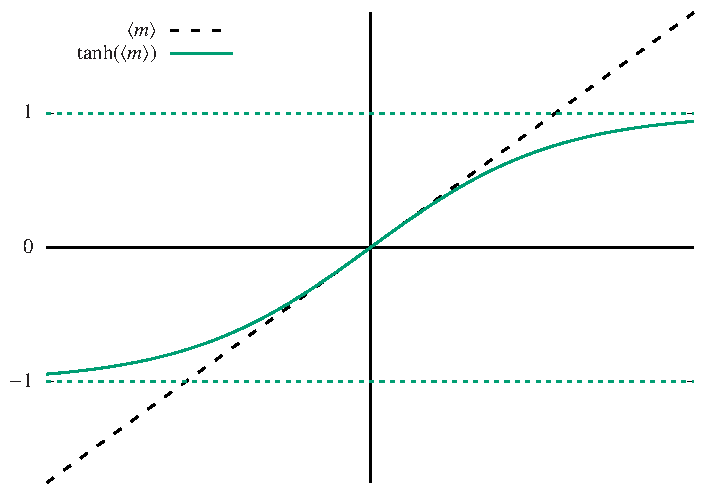
\includegraphics[width=0.7\textwidth]{figs/unit09_consistency.pdf}\end{center}

To confirm our interpretation of this result, let's check how the intersections depend on \be and $H$.
In the next plot below we keep the same temperature $T = 1 / \be = 4$ while comparing two non-zero values for the external magnetic field.
A positive $H = 2$ simply shifts $g(\vev{m})$ to the left (the green line), while a negative $H = -2$ shifts it to the right (the blue line).
In both cases there is still only a single intersection, at $\vev{m} \approx \pm 0.88$ for $H = \pm 2$.
We can interpret this non-zero result as an indication that the system is in an ordered phase where the spins tend to align with the external field. \\[-24 pt]
\begin{center}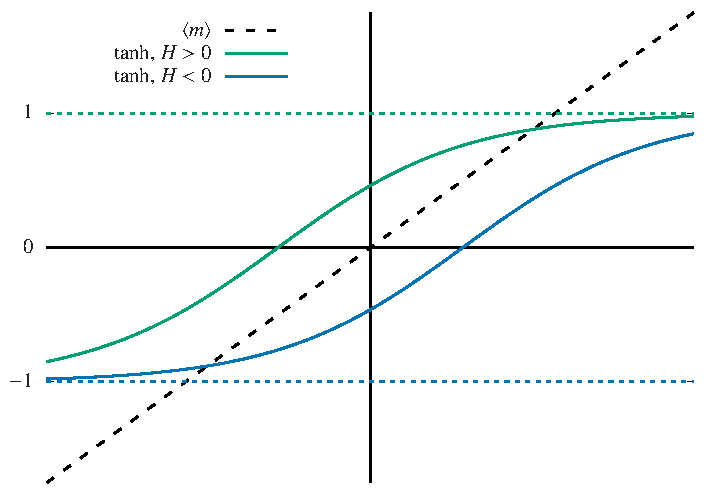
\includegraphics[width=0.69\textwidth]{figs/unit09_consistency_H.pdf}\end{center} % WARNING: ADJUSTED SIZE BY HAND TO FIT BOTH ON PAGE

From our work in the previous section, we can expect that the spins' alignment will increase --- approaching the minimal-energy ground state --- as the temperature decreases.
Decreasing the temperature increases $\be$, which causes the argument of the $\tanh$ to vary more rapidly with $\vev{m}$, making $g(\vev{m})$ a steeper function that more rapidly approaches its limiting values $\pm 1$.
The plot below illustrates this for $T = 1 / \be = 2$, so that $\be = \frac{1}{2}$ is doubled.
Already for this temperature and magnetic field $H = \pm 2$, the intersection is $\vev{m} \approx \pm 1$ to a very good approximation.
We can also appreciate that $-1 \leq \tanh x \leq 1$ ensures that the mean-field self-consistency condition can only ever be satisfied for $-1 \leq \vev{m} \leq 1$, reassuringly consistent with the definition of the magnetization. \\[-24 pt]
\begin{center}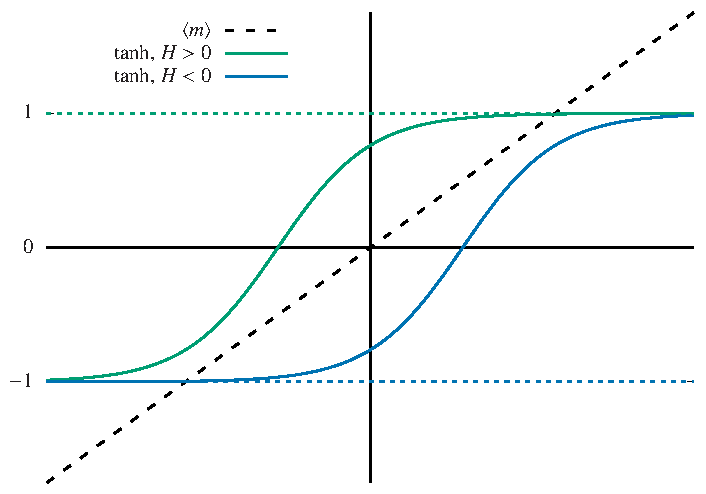
\includegraphics[width=0.69\textwidth]{figs/unit09_consistency_H-beta.pdf}\end{center} % WARNING: ADJUSTED SIZE BY HAND TO FIT BOTH ON PAGE

Also in the previous section, we saw that the Ising model spins should align at low temperatures, even without an external field to promote one direction over the other.
We hope to see this behaviour captured by the mean-field approximation, which we can check by considering the self-consistency condition for various temperatures with $H = 0$.
The plot below shows the results, considering a low temperature $T = 2$ with $\be = \frac{1}{2}$ (the blue line), the same green curve for $T = 4$ shown in the first plot above, and a high temperature $T = 8$ with $\be = \frac{1}{8}$ (the red line).
While the $\vev{m} = 0$ expected in the disordered phase is always a possible solution, something interesting happens at lower temperatures, where the steeper $\tanh$ function introduces two additional solutions at non-zero $\vev{m} = \pm m_0$ corresponding to the ordered phase.
As $T \to 0$, this magnetization approaches its maximum value $m_0 \to 1$.

\begin{center}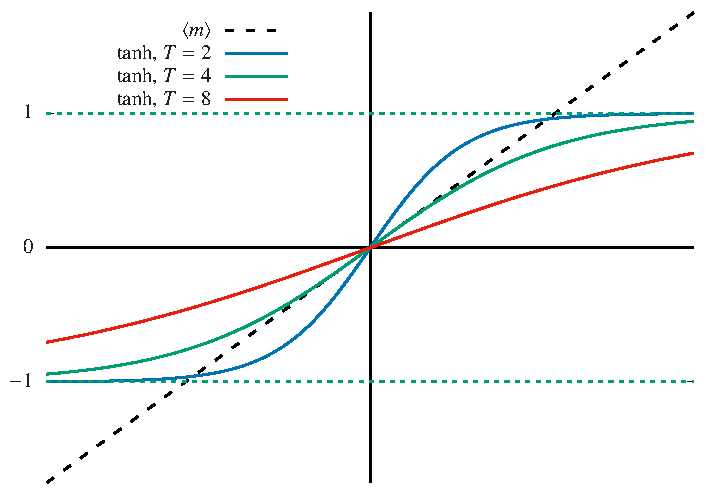
\includegraphics[width=0.7\textwidth]{figs/unit09_consistency_beta.pdf}\end{center}

When there are three solutions $\vev{m} = \left\{-m_0, 0, m_0\right\}$ at low temperatures, we can determine that the $\vev{m} = 0$ solution is actually \textit{unstable}.
Here we are venturing briefly into non-equilibrium territory, and thinking of the mean-field system as a `blind' process that attempts to satisfy the self-consistency condition $\vev{m} = \tanh\left[2\be d\vev{m}\right]$, based only on knowledge of whether the expectation value of the magnetization is too small or too large compared to the $\tanh$. % TODO: Changing expectation value sign of non-equilibrium... Could mention `quenches'...
Once the magnetization is self-consistent, the system can happily settle into thermodynamic equilibrium.

From the figure above we can see that (with $H = 0$) we can have three solutions only when the slope of the $\tanh$ at $\vev{m} = 0$ is greater than $1$. % TODO: Need at least one for asymptotic consistency...
Any positive value $\vev{m} = \varepsilon > 0$ would then produce $\tanh\left[2\be d\vev{m}\right] > \vev{m}$, which the system `feels' as a magnetization that is too small to be self-consistent.
This drives the system to continue increasing its magnetization, until it eventually settles at the non-zero solution $\vev{m} = m_0$.
Similarly, any negative magnetization $\vev{m} = -\varepsilon < 0$ would drive $\vev{m}$ away from zero and to the $\vev{m} = -m_0$ solution.

This argument can be visualized more easily by plotting $\tanh\left[2\be d\vev{m}\right] - \vev{m}$ vs.\ $\vev{m}$ as shown in the final plot below.
Whenever this difference is negative, it implies $\vev{m}$ is larger than the self-consistency condition allows, driving the system to smaller $\vev{m}$ as shown by the arrows pointing to the left.
Conversely, whenever the difference is positive, the system `seeks' self-consistency by increasing $\vev{m}$ as shown by the arrows pointing to the right.
For the low temperature $T = 2$, we see that the arrows move the system away from the unstable solution $\vev{m} = 0$ and to the stable solutions $\vev{m} = \pm m_0$.

\begin{center}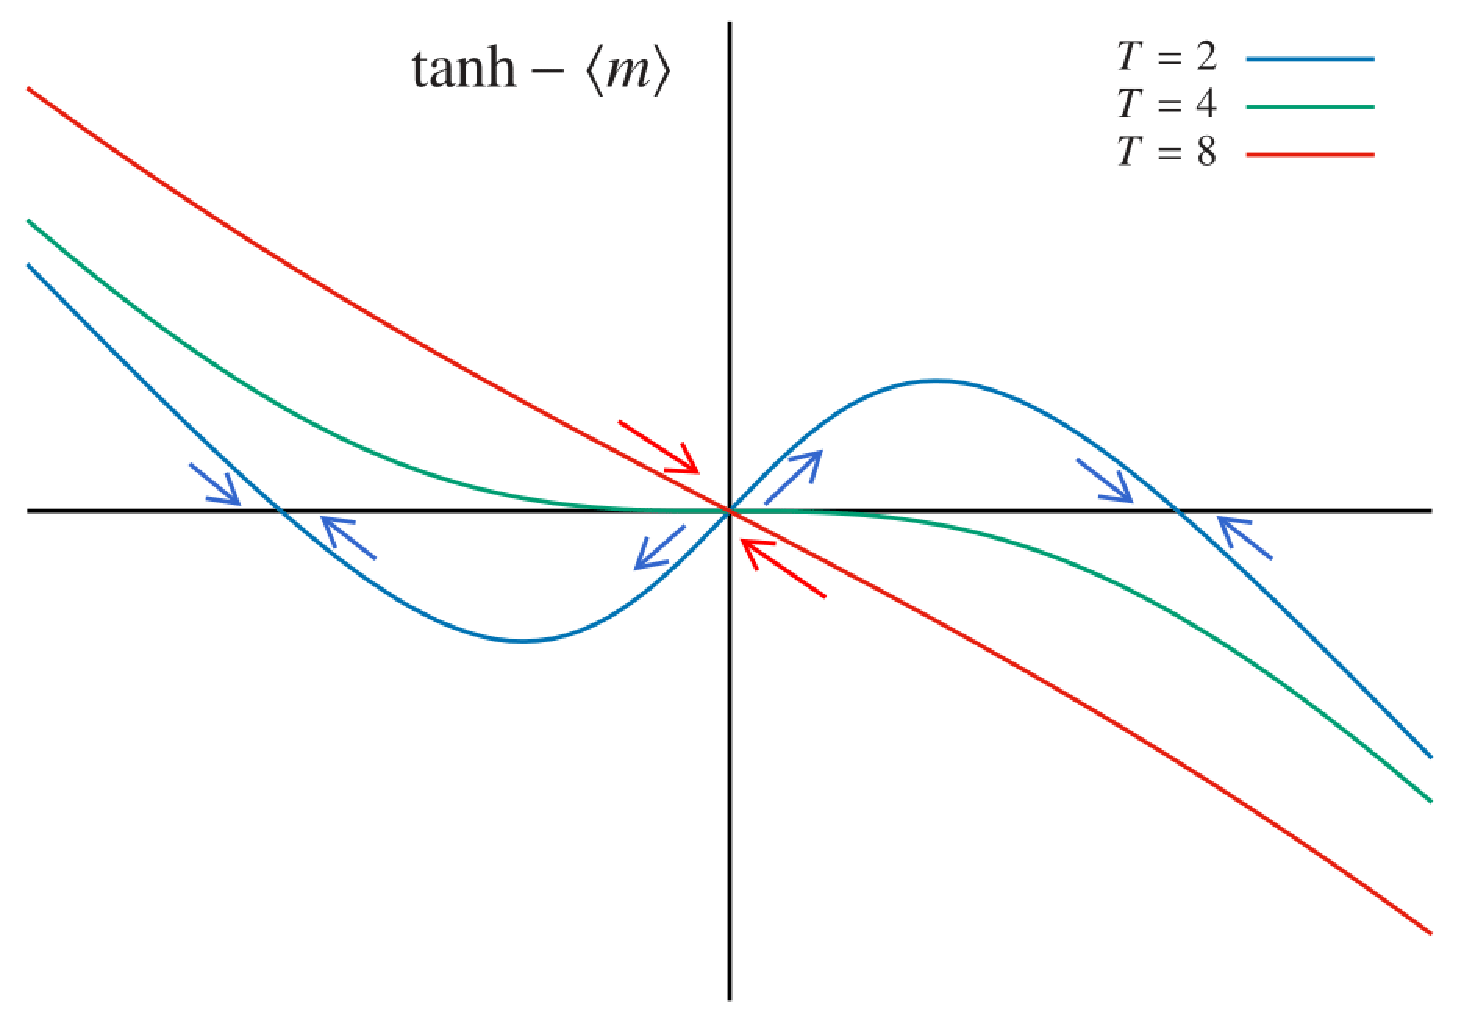
\includegraphics[width=0.7\textwidth]{figs/unit09_consistency_flow.pdf}\end{center}

So in the end we can conclude that the non-interacting mean-field approximation successfully captures at least the high- and low-temperature limits of the interacting zero-field Ising model that we determined in the previous section.
For high temperatures the mean-field self-consistency condition demands $\vev{m} = 0$ consistent with the disordered phase, while for low temperatures it produces $|\!\vev{m}\!| = m_0 > 0$ consistent with the ordered phase. % TODO: Note $|\!\vev{m}\!|$ vs.\ $\vev{|m|}$...

Going further, now that we have a more tractable non-interacting system we can consider the value of the temperature at which the $\vev{m} = \pm m_0$ solutions appear and the $\vev{m} = 0$ solution becomes unstable.
As described above, this occurs whenever the slope of the $\tanh$ function at $\vev{m} = 0$ is greater than $1$.
Let's call the corresponding temperature $T_c$, though it remains to be determined whether it is really a critical temperature of a true phase transition.
Expanding $\tanh(x) = x + \cO\left(x^3\right)$ for $x \approx 0$, what is $T_c$?
\begin{mdframed}
  \ \\[50 pt]
\end{mdframed}

You should find that the change from the high-temperature disordered phase to the low-temperature ordered phase occurs at $T_c = 2d$ in $d$ dimensions, or equivalently $\be_c = \frac{1}{2d}$ --- corresponding to the green lines in the two figures above with $d = 2$.
In order to determine whether or not this is a true critical temperature, we need to check whether the order parameter $\vev{m}$ or its $T$-derivatives are discontinuous at $T_c$.
We can do this by considering the self-consistency condition for a temperature $T$ lower than but very near to $T_c = 2d$, which would produce $0 < |\vev{m}| \ll 1$ and allow us to expand $\tanh(x) = x - \frac{x^3}{3} + \cO\left(x^5\right)$.
What is the resulting prediction for $\vev{m}$?
\begin{mdframed}
  \ \\[100 pt]
\end{mdframed}

Making the approximation $\left(\frac{T}{T_c}\right)^2 \approx 1$, your result should resemble
\begin{equation*}
  \vev{m} = \pm \sqrt{3} \left(\frac{T_c - T}{T_c}\right)^{1 / 2} \qquad \mbox{for } \ T \lesssim T_c.
\end{equation*}
From this, we can see that the order parameter $\vev{m}$ is continuous at $T_c$:
\begin{equation}
  \vev{m} \propto \left\{\begin{array}{cl} \left(T_c - T\right)^{1 / 2} & \mbox{for } \ T \lesssim T_c \\[3 pt]
                                           0                            & \mbox{for } \ T \gtrsim T_c\end{array}\right. .
\end{equation}
However, its first derivative
\begin{equation*}
  \frac{d\vev{m}}{dT} \propto \frac{1}{\left(T_c - T\right)^{1 / 2}}
\end{equation*}
diverges as $T \to T_c$ from below.
This is the situation we discussed at the end of the previous section, which predicts a second-order phase transition with critical temperature $T_c = 2d$ in $d$ dimensions.
The power-law dependence $\vev{m} \propto \left(T_c - T\right)^b$ with \textit{non-integer} $b$ is a generic feature of second-order phase transitions. % TODO: With integer $b$, derivatives flatten and eventually vanish...
The power $b$ is known as a \textbf{critical exponent}, in this case $b = 1 / 2$.

At this point we have invested some effort to find that the mean-field approximation of the $d$-dimensional Ising model, with $H = 0$, predicts a second-order phase transition at $T_c = 2d$ with critical exponent $1 / 2$.
Let's wrap up this section with some quick comments on the reliability of the mean-field approximation and the accuracy of these results it has given us.

The accuracy of the mean-field results turns out to depend on the number of dimensions.
For the one-dimensional Ising model that Ising himself solved, there is no phase transition at all, as we will derive in the next section.
In other words, the mean-field approximation simply fails for $d = 1$.

The situation improves for the two-dimensional Ising model.
Onsager's exact $H = 0$ solution features a second-order phase transition, at an inverse critical temperature $\be_c = \frac{1}{2} \log\left(1 + \sqrt{2}\right) \approx 0.44$ that had been exactly determined a few years before his work.
For $T \lesssim T_c$, the magnetization vanishes as $\vev{m} \propto \left(T_c - T\right)^{1 / 8}$, corresponding to a critical exponent $1 / 8$.
While the mean-field prediction of a second-order phase transition is now qualitatively correct, at a quantitative level its predicted $\be_c = \frac{1}{2d} = 0.25$ is off by almost a factor of $2$, while the mean-field critical exponent $b = 1 / 2$ is four times larger than the true $b = 1 / 8$.

For higher dimensions $d \geq 3$ there is no known exact solution for the Ising model, but the existence of a second-order phase transition can be established and the corresponding critical temperature and critical exponents can be computed numerically, as we will discuss in Unit~10.
In three dimensions the mean-field $T_c = 2d = 6$ and $b = 1 / 2$ are still significantly different from the true $T_c \approx 4.5$ and $b \approx 0.32$. % From Tong and arXiv:1806.03558
The mean-field prediction for the critical exponent $b = 1 / 2$ turns out to be correct for $d \geq 4$, while the critical temperature $T_c = 2d$ gradually approaches the true value as the number of dimensions increases.
Numerical computations find $T_c \approx 6.7$, $8.8$, $10.8$ and $12.9$ for $d = 4$, $5$, $6$ and $7$, respectively, so that the mean-field result improves from being $\sim$$19\%$ too high for $d = 4$ to only $\sim$$9\%$ too high for $d = 7$. % From arXiv:1202.3031 and arXiv:1502.07613
Formally, the mean-field approximation exactly reproduces the Ising model in the abstract limit of infinite dimensions, $d \to \infty$.
Roughly speaking, the greater reliability of the mean-field approach in higher dimensions is due to the larger number of nearest neighbours for each site, $2d$.
The larger number of nearest-neighbour spins produces a more reliable approximation of the mean spin in the effective field seen by each site in the mean-field approach.
% ------------------------------------------------------------------



% ------------------------------------------------------------------
\subsection{Exact results for the Ising model}
If time permits, it is not too hard to prove some of the exact results mentioned above, for the Ising model in one and two dimensions where the mean-field approximation is least reliable.

\subsubsection{One-dimensional partition function and magnetization}
The special property of the one-dimensional Ising model that helps us derive a closed-form expression for its partition function is the fact that it has exactly as many links as it has sites.
Looking back to the illustration on page~134, we can rewrite the nearest-neighbour interaction term as
\begin{equation*}
  \sum_{(jk)} s_j s_k = \sum_{n = 1}^N s_n s_{n + 1},
\end{equation*}
where the periodic boundary conditions identify $s_{N + 1} = s_1$.
If we also rewrite $H \sum_{n = 1}^N s_n = \frac{H}{2} \sum_{n = 1}^N \left(s_n + s_{n + 1}\right)$, then the full internal energy is
\begin{equation*}
  E_i = -\sum_{n = 1}^N \left[s_n s_{n + 1} + \frac{H}{2}\left(s_n + s_{n + 1}\right)\right].
\end{equation*}
Inserting this into the partition function $Z(\be, N, H) = \sum_{\left\{s_n\right\}} \exp\left[-\be E(s_n)\right]$, we can convert the exponential of the sum into a product of exponentials,
\begin{equation*}
  Z = \sum_{s_1 = \pm 1} \cdots \sum_{s_N = \pm 1} \prod_{n = 1}^N \exp\left[\be s_n s_{n + 1} + \frac{\be H}{2}\left(s_n + s_{n + 1}\right)\right].
\end{equation*}

Similarly to \eq{eq:spin_part_func} for the non-interacting case, we are going to distribute the summations.
Now, however, we have to keep track of the fact that a given spin $s_j$ will appear both when $n = j$ and when $n + 1 = j$, and for each spin configuration it must have the same value both times it appears.
An elegant way to account for all allowed possibilities is through matrix multiplication.
Use the $2\times 2$ matrix
\begin{equation}
  T_n = \begin{pmatrix} e^{\be + \be H} & e^{-\be} \\ e^{-\be} & e^{\be - \be H} \end{pmatrix}
\end{equation}
to collect the exponential factors for the four possibilities
\begin{equation*}
  \left\{s_n, s_{n + 1}\right\} = \begin{pmatrix} \left\{1, 1\right\} & \left\{1, -1\right\} \\ \left\{-1, 1\right\} & \left\{-1, -1\right\} \end{pmatrix}.
\end{equation*}
The matrix product $T_n \cdot T_{n + 1}$ then provides the sum over all contributions with consistent values for $s_{n + 1}$.
Repeating this for all terms in $\prod_{n = 1}^N$, the periodic boundary conditions produce the (cyclic) trace, making the exact partition function simply
\begin{equation*}
  Z = \mbox{Tr}\left[\prod_{n = 1}^N T_n \right].
\end{equation*}
What's more, since $T_n \equiv T$ is actually independent of $n$, this simplifies further to
\begin{equation}
  Z = \mbox{Tr}\left[T^N \right].
\end{equation}

$T$ is known as the \textbf{transfer matrix} --- roughly speaking, it `transfers' information about the values of the spins from one link to the next.
At this point we can appreciate that our earlier rewriting of the magnetic-field term in the energy just helped to make $T$ more symmetric.
If we now diagonalize
\begin{equation*}
  T = \begin{pmatrix} e^{\be} e^{\be H} & e^{-\be} \\ e^{-\be} & e^{\be} e^{-\be H} \end{pmatrix} \quad \lra \quad \begin{pmatrix} \la_+ & 0 \\ 0 & \la_- \end{pmatrix},
\end{equation*}
the partition function will become simply
\begin{equation*}
  Z = \mbox{Tr}\left[\begin{pmatrix} \la_+ & 0 \\ 0 & \la_- \end{pmatrix}^N\right] = \mbox{Tr}\begin{pmatrix} \la_+^N & 0 \\ 0 & \la_-^N \end{pmatrix} = \la_+^N + \la_-^N.
\end{equation*}
\newpage % WARNING: FORMATTING BY HAND
\noindent What are the two eigenvalues $\la_{\pm}$ of $T$?
\begin{mdframed}
  \ \\[100 pt]
\end{mdframed}

With $\be \geq 0$ and $H \geq 0$, we can check that both eigenvalues are real and $\la_+ > \la_-$.
For asymptotically high temperatures, $\be \to 0$, the eigenvalues reduce to $\la_+ = 2$ and $\la_- = 0$ independent of $H$.
In the special case $H = 0$, the eigenvalues are $\la_+ = 2\cosh\be$ and $\la_- = 2\sinh\be$, while $H > 0$ typically produces $\la_+ \gg \la_-$.
Because $\la_- / \la_+ < 1$, for sufficiently large $N \gg 1$ we can further simplify
\begin{equation*}
  Z = \la_+^N\left[1 + \left(\frac{\la_-}{\la_+}\right)^N \right] \approx \la_+^N = e^{N\be} \cosh^N(\be H)\left[1 + \sqrt{1 - \frac{2\sinh(2\be)}{e^{2\be}\cosh^2(\be H)}}\right]^N.
\end{equation*}

So there we have it --- the solution of the Ising model in one dimension.
As usual, the partition function $Z$ is not so revelatory in and of itself.
Its principal value lies in enabling us to predict observables like the magnetization --- so let's do that, returning to the zero-field case for which we computed the mean-field critical temperature and critical exponent in the previous section:
\begin{mdframed}
  $\displaystyle \vev{m} = \left. \frac{1}{N\be} \pderiv{}{H}\log Z \right|_{H = 0} = $ \\[80 pt]
\end{mdframed}
Note that we set $H = 0$ only \textit{after} computing the derivative of the free energy, which avoids the need to consider the absolute value.
Upon setting $H = 0$, something remarkable happens: $\vev{m} = 0$ for all temperatures!

As claimed at the end of the previous section, the one-dimensional Ising model has no phase transition at all.
It is always in the disordered phase, even in the limit of absolute zero $T \to 0$.
In addition to revealing that the mean-field approximation fails in one dimension, this result also shows how the balance of energy level degeneracy vs.\ Boltzmann factor considered in \secref{sec:Ising_phases} depends on the lattice structure.

For the case of a one-dimensional lattice, the first excited energy level with energy $E_1$ includes more micro-states than the $2N$ we get by flipping a single spin to oppose the full alignment of the ground state.
Suppose we start from the ground state and flip spin $s_j$ to reach the first excited energy level.
Relative to the ground-state energy $E_0 = -N$, the energy of this micro-state is increased to $E_1 = -N + 4$ due to the positive contributions from the $s_{j - 1} s_j$ and $s_j s_{j + 1}$ links.
But if we now consider \textit{also} flipping spin $s_{j + 1}$, the $s_j s_{j + 1}$ link goes back to providing a negative contribution while the positive contribution shifts to the $s_{j + 1} s_{j + 2}$ link.
This gives us an additional $2N$ micro-states featuring a flipped nearest-neighbour \textit{pair} of spins, with the same energy $E_1$ but a smaller magnetization $|m| = 1 - \frac{4}{N}$.
And we can continue this process, finding more degenerate micro-states with a flipped block of \textit{any} number of neighbouring spins up to $N - 1$, and hence any magnetization, including $m = 0$.

The non-existence of an ordered phase in one dimension also holds for more general interacting systems beyond just the Ising model.
A useful way to analyze this sort of behaviour is to describe all of the micro-states in the first excited energy level as consisting of two \textit{domains} separated by two \textbf{domain walls} (recalling the periodic boundary conditions).
For the Ising model, one domain will contain only up spins while the other will contain only down spins.
The two domain walls are able to move freely through the lattice without changing the energy, but as the domain walls move the magnetization samples the full range of values $-\left(1 - \frac{2}{N}\right) \leq m \leq 1 - \frac{2}{N}$.

\subsubsection{Two-dimensional critical temperature}
While the zero-field Ising model on the $d = 2$ square lattice has also been exactly solved, both Onsager's original calculation and subsequent re-derivations using simpler techniques go substantially beyond this module.
However, a few years before Onsager published his famous result, \href{https://en.wikipedia.org/wiki/Hans_Kramers}{Hans Kramers} and \href{https://en.wikipedia.org/wiki/Gregory_Wannier}{G.~H.~Wannier} were able to determine the exact $d = 2$ critical temperature \href{https://doi.org/10.1103/PhysRev.60.252}{in 1941}.
They did this by identifying a relation between two Ising model partition functions, without actually evaluating either sum over micro-states:
\begin{equation}
  \label{eq:dual_Z}
  \frac{Z(\be)}{2^N \cosh^{2N} \be} = \frac{Z(\betw)}{2e^{2N\betw}},
\end{equation}
where the two inverse temperatures \be and \betw are related by
\begin{equation}
  \label{eq:dual_beta}
  \sinh(2\be) = \frac{1}{\sinh(2\betw)}.
\end{equation}
This relation is now known as \href{https://en.wikipedia.org/wiki/Kramers-Wannier_duality}{Kramers--Wannier duality}, and the general concept of duality has become a powerful tool in modern theoretical physics.
Note that small \be implies large \betw and vice versa --- the duality relates one $d = 2$ Ising model at a high temperature to another one at a low temperature.

Although it can be instructive to explicitly compare such high- and low-temperature partition functions, by computing series expansions as we did for the non-interacting spin system in \secref{sec:spin_info} and for the Einstein solid in a tutorial, to keep this section under control I'll skip that exercise.
Those who are interested can find related discussions in Sections~5.3.2 and 5.3.3 of David Tong's \href{https://www.damtp.cam.ac.uk/user/tong/statphys.html}{\textit{Lectures on Statistical Physics}} (the first item in the list of further reading on page~6).
Some of the manipulations below, which may seem to come out of thin air, can be motivated by considering these expansions.

The first manipulation is to express the zero-field partition function as
\begin{equation*}
  Z = \sum_{\left\{s_n\right\}} \exp\left[\be\sum_{(jk)} s_j s_k\right] = \sum_{\left\{s_n\right\}} \prod_{(jk)} \exp\left[\be s_j s_k\right] = \sum_{\left\{s_n\right\}} \prod_{(jk)} \left[\cosh \be + s_j s_k \sinh \be\right],
\end{equation*}
which relies on the fact $s_j s_k = \pm 1$ for the Ising model.
It's easy to check the relation $e^{\be s_j s_k} = \cosh \be + s_j s_k \sinh \be$ for both cases:
\begin{mdframed}
  \ \\[60 pt]
\end{mdframed}
Next, we write the sum over the $\cosh$ and $\sinh$ as an explicit summation,
\begin{equation*}
  Z = \sum_{\left\{s_n\right\}} \prod_{(jk)} \left[\cosh \be + s_j s_k \sinh \be\right] = \sum_{\left\{s_n\right\}} \prod_{(jk)} \sum_{p_{jk} = 0, 1} C_{p_{jk}}(\be) (s_j s_k)^{p_{jk}},
\end{equation*}
raising $s_j s_k$ to the corresponding power $p_{jk}$ while defining $C_0(\be) \equiv \cosh \be$ and $C_1(\be) \equiv \sinh \be$.
Recall that the sum over nearest-neighbour pairs $(jk)$ corresponds to summing over all $2N$ links in the $d = 2$ lattice.
To make the language a little less awkward, we can say that $p_{jk} = 1$ corresponds to link $jk$ being `on' while $p_{jk} = 0$ when it is turned `off'.
The product and sum above account for all possible configurations of links that are turned on and off, which we can more conveniently represent as another configuration sum,
\begin{equation*}
  \sum_{\left\{p\right\}} \equiv \sum_{p_1 = 0, 1} \cdots \sum_{p_{2N} = 0, 1}.
\end{equation*}

Introducing this configuration sum lets us isolate and then trivially rearrange the final product,
\begin{equation*}
  Z = \sum_{\left\{s_n\right\}} \sum_{\left\{p\right\}} \prod_{(jk)} C_{p_{jk}}(\be) (s_j s_k)^{p_{jk}} = \sum_{\left\{s_n\right\}} \sum_{\left\{p\right\}} \left[\prod_{(jk)} C_{p_{jk}}(\be)\right] \left[\prod_{(jk)} s_j^{p_{jk}} s_k^{p_{jk}}\right].
\end{equation*}
The final factor can now be converted from a product over links to a product over sites.
Any given spin $s_n$ will appear four times in the product, once for each of the four links connected to it in two dimensions.
The product of these four factors can be rewritten
\begin{align*}
  \prod_{(nk)} s_n^{p_{nk}} & = s_n^{P_n}, &
  \mbox{defining } \ P_n & \equiv \sum_{(nk)} p_{nk}.
\end{align*}

We are now left with a product over individual $s_n$:
\begin{equation*}
  Z = \sum_{\left\{p\right\}} \prod_{(jk)} C_{p_{jk}}(\be) \sum_{\left\{s_n\right\}} \prod_{n = 1}^N s_n^{P_n}.
\end{equation*}
Although each $s_n$ is raised to a power that depends on $p_{nk}$ for all four of its links to its nearest neighbours, and can consider what happens when we sum over the two values $s_n = \pm 1$.
There are two possibilities: If $P_n$ is odd, then the $s_n = 1$ and $s_n = -1$ contributions cancel --- making the entire product over sites vanish!
Otherwise, if $P_n$ is even, they add up to $2$.
In other words, we have
\begin{equation}
  \label{eq:constrained_Ising}
  Z = \sum_{\left\{p\right\}} \prod_{(jk)} C_{p_{jk}}(\be) \prod_{n = 1}^N 2\de_2(P_n) = 2^N \sum_{\left\{p\right\}} \prod_{(jk)} C_{p_{jk}}(\be) \prod_{n = 1}^N \de_2\left(\Sigma_{(nk)} p_{nk}\right),
\end{equation}
where the `mod-$2$' Kronecker delta $\de_2(P_n)$ vanishes if $P_n$ is odd and equals one if $P_n$ is even.

Something interesting has happened in \eq{eq:constrained_Ising}: there is no longer any reference to our original spin degrees of freedom, $s_n$.
We have successfully summed over all spin configurations $\left\{s_n\right\}$, at the cost of introducing a different sum over all configurations of on/off links ($p_{jk} = 1$ or $0$, respectively).
And there is a very tricky set of $N$ inter-dependent constraints coming from the product of $\de_2$ factors, which require that an even number of links be turned on at \textit{every} lattice site, in order to get a non-zero contribution to the partition function.
In effect, this informs us that our new variables $p_{jk}$ aren't really independent of each other --- which makes sense, since we have $2N$ of them, but started off with only $N$ degrees of freedom.

What we can do about this is essentially to try working backwards.
We introduced the $p_{jk} = 0, 1$ in order to manipulate a configuration sum over $s_n = \pm 1$, so we can guess that introducing a different set of $\stw_n = \pm 1$ can have an effect on the resulting configuration sum over $p_{jk}$.
We want the $\pm 1$ values of $\stw_n$ to be related to the $\left\{0, 1\right\}$ values of $p_{jk}$, which we can achieve by implicitly defining $\stw_n$ via
\begin{align*}
  p_{12} & = \frac{1 - \stw_1 \stw_2}{2} &
  p_{13} & = \frac{1 - \stw_2 \stw_3}{2} \\
  p_{14} & = \frac{1 - \stw_3 \stw_4}{2} &
  p_{15} & = \frac{1 - \stw_1 \stw_4}{2}
\end{align*}
and so on for all $2N$ links.
A convenient way to keep track of the subscripts above is to identify these $\stw_n$ with the \textbf{dual lattice} drawn on the next page.
Each $\stw_n$ is identified with one of the $N$ plaquettes of the original lattice, and pairs $\stw_a$ and $\stw_b$ determine $p_{jk}$ for the link passing between them.

\begin{center}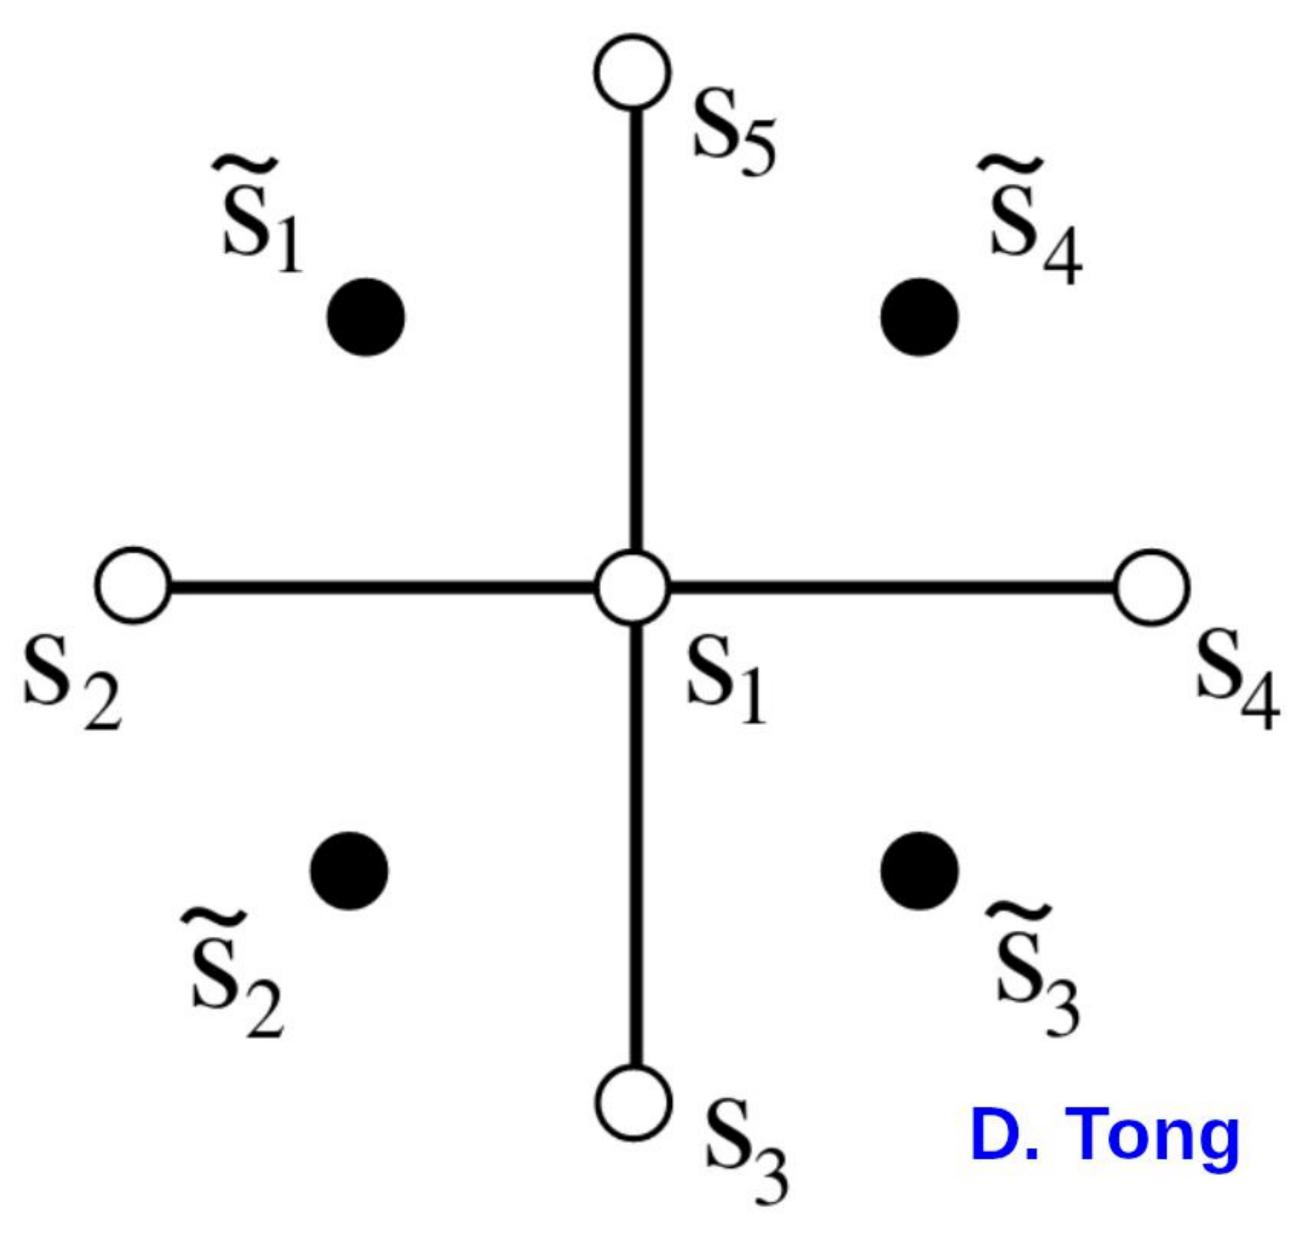
\includegraphics[width=0.5\textwidth]{figs/unit09_dual_lattice.pdf}\end{center}

These relations confirm the claim above that $p_{jk}$ aren't independent variables --- both $p_{12}$ and $p_{15}$ depend on $\stw_1$, both $p_{12}$ and $p_{13}$ depend on $\stw_2$, etc.
Delightfully, these patterns of dependence are precisely what we need to handle the $\de_2$ factors that are still in our partition function.
If we consider
\begin{align*}
  P_1 & = p_{12} + p_{13} + p_{14} + p_{15} = 2 - \frac{\stw_1 \stw_2 + \stw_2 \stw_3 + \stw_3 \stw_4 + \stw_1 \stw_4}{2} \\
      & = 2 - \frac{(\stw_1 + \stw_3)(\stw_2 + \stw_4)}{2} \in \left\{0, 2, 4\right\},
\end{align*}
we see that working in terms of $\stw_n$ automatically turns on an even number of links at every site, producing $\prod_{n = 1}^N \de_2(P_n) = 1$!

In addition to eliminating odd $P_1$, you can confirm that all possible ways of obtaining even $P_1$ are accounted for as configurations of the dual spins $\stw_n$.
In fact, they all appear twice, as we can see by checking the simple example $P_1 = 4$: % TODO: 1+6+1 ways of getting P_1 = 0, 2, 4 account for all 2+12+2=16 = 2^4 combinations of spins...
\begin{mdframed}
  \ \\[50 pt]
\end{mdframed}
This generalizes to the full $N$-spin system,\footnote{This is discussed in more detail by Robert Savit, ``\href{https://doi.org/10.1103/RevModPhys.52.453}{Duality in field theory and statistical systems}'', \textit{Reviews of Modern Physics} \textbf{52}:453, 1980} so converting the partition function from the configuration sum over $\left\{p\right\}$ in \eq{eq:constrained_Ising} to a configuration sum over $\left\{\stw\right\}$ gives us
\begin{equation*}
  Z = \frac{1}{2} 2^N \sum_{\left\{\stw\right\}} \prod_{(jk)} C_{(1 - \stw_j \stw_k) / 2}(\be).
\end{equation*}

The final step is to express
\begin{align*}
  C_0(\be) & = \cosh \be &
  C_1(\be) & = \sinh \be
\end{align*}
in terms of the dual variables $\stw_n$ that we're now working with.
It's easy to see that
\begin{equation*}
  C_p(\be) = \left(\cosh \be\right) \exp\left[p \log \tanh \be\right] = \left(\cosh \be\right) \exp\left[\frac{1 - \stw_j \stw_k}{2} \log \tanh \be\right],
\end{equation*}
substituting $p = (1 - \stw_j \stw_k) / 2$.
Breaking up the exponential gives us
\begin{equation*}
  C_p(\be) = \left(\cosh\be \sinh\be\right)^{1 / 2} \exp\left[-\frac{1}{2} \stw_j \stw_k \log \tanh \be\right].
\end{equation*}
Inserting this into the partition function, the product over all links just provides $2N$ factors of the $\stw_n$-independent first term, and we can then convert the product of exponentials into an exponential of the sum, producing
\begin{equation*}
  Z = \frac{1}{2} \left(2\cosh\be \sinh\be\right)^N \sum_{\left\{\stw\right\}} \exp\left[-\frac{\log \tanh \be}{2} \sum_{(jk)} \stw_j \stw_k\right].
\end{equation*}

If we define
\begin{equation*}
  \betw \equiv -\frac{\log \tanh \be}{2},
\end{equation*}
then we can recognize the sum over $\left\{\stw\right\}$ configurations as simply a zero-field Ising model partition function $Z(\betw)$ as in \eq{eq:Ising_zero_field}.
We can also recognize this definition of \betw as equivalent to \eq{eq:dual_beta}:
\begin{mdframed}
  \ \\[100 pt]
\end{mdframed}
Using similar manipulations, we can express the spin-independent prefactor in terms of either \be or $\betw$,
\begin{equation*}
  2\cosh\be \sinh\be = \sinh(2\be) = \frac{1}{\sinh(2\betw)},
\end{equation*}
or in the mixed form that reproduces \eq{eq:dual_Z}:
\begin{equation*}
  2\cosh\be \sinh\be = 2\cosh^2 \be \tanh\be = \frac{2\cosh^2 \be}{e^{2\betw}} \quad \implies \quad \frac{Z(\be)}{\left(2\cosh^2\be\right)^N} = \frac{Z(\betw)}{2e^{2N\betw}}.
\end{equation*}

We have successfully derived Kramers--Wannier duality!
Now let's briefly interpret what it means.
It's a worthwhile \textbf{exercise} to show that multiplying a partition function by an overall spin-independent factor, $Z(\be) \to c(\be) Z(\be)$, has no effect on expectation values.
(Try it!)
Therefore the relation above identifies a $d = 2$ Ising system at temperature \be with another such system at temperature $\betw$, where small \be corresponds to large \betw and vice versa.

However, this does \textit{not} mean that $d = 2$ Ising model behaves the same at low and high temperatures.
Indeed, we saw already in \secref{sec:Ising_phases} that it changes between qualitatively different ordered and disordered phases in these two regimes.
What Kramers--Wannier duality is telling us is that the ordered phase of Ising spins in two dimensions, characterized by their order parameter, is secretly equivalent to the disordered phase of the \textit{dual} spins --- a different set of degrees of freedom, which can be characterized by a `disorder parameter'.
Similarly, the disordered phase of the original system maps onto the ordered phase of the dual system.

If we assume there is a single phase transition where the ordered and disorederd phases coincide, then Kramers--Wannier duality implies this must occur when $\be = \betw$.
In other words,
\begin{equation*}
  \sinh^2(2\be_c) = 1 \quad \Lra \quad \be_c = \frac{1}{2} \mathrm{arcsinh}(1) = \frac{\log\left(1 + \sqrt{2}\right)}{2} = 0.440686\dots,
\end{equation*}
recalling (or looking up) that $\mathrm{arcsinh}(x) = \log\left(x + \sqrt{x^2 + 1}\right)$.
Because this exact critical temperature $T_c = 2 / \log\left(1 + \sqrt{2}\right) = 2.269185\dots$ was predicted three years before Onsager analytically solved the $d = 2$ Ising model, the fact that his solution correctly reproduced this $T_c$ was a significant check of its correctness.

As mentioned at the start of this subsection, dualities of this sort are a pillar of theoretical physics in the 21st century.
In general, these dualities are much more complicated than Kramers--Wannier duality, in two main ways.
First, the dual degrees of freedom are typically different --- and have different interactions --- than the original degrees of freedom.
For example, if we were to carry out a similar analysis of the three-dimensional Ising model, we would find that the dual system is \textit{not} just another Ising model. % TODO: It is a Z2 gauge theory, sometimes (perhaps confusingly) called an `Ising gauge model'...
The $d = 2$ Ising model is a special case of a \textbf{self-dual} system, which we exploited to determine $T_c$.

Second, the Ising model is special in that we were able to explicitly derive the duality it exhibits, which is typically not (yet) possible.
Instead, most dualities have to be conjectured and then checked by subjecting them to as many tests as possible.
For example, this is the case for \textit{holographic dualities} that are conjectured to relate certain theories of quantum gravity to non-gravitational quantum systems that can be much easier to analyze mathematically.
As an aside, the fully connected lattice we encountereed in recent tutorials also makes an appearance in holography --- the behaviour of interacting fermions on this fully connected lattice (known as the \href{https://en.wikipedia.org/wiki/Sachdev-Ye-Kitaev_model}{SYK model}, named after Subir Sachdev, Jinwu Ye and Alexei Kitaev) is conjected to be dual to the gravitational dynamics of quantum black holes.
\href{https://inspirehep.net/literature/342314}{More than a thousand} scientific studies related to the SYK model and its conjectured holographic duality have been published since 2016!
% ------------------------------------------------------------------
